Der Körper $\mathbb{F}_2$ ist besonders einfach, da er nur zwei Elemente
$0$ und $1$ enthält.
Die Additions- und Multiplikationstabellen sind
\begin{center}
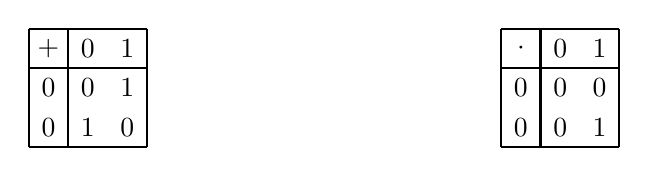
\begin{tikzpicture}[>=latex,thick]
\def\ds{0.5}
\def\punkt#1#2{({(#1)*\ds},{(-#2)*\ds})}
\def\tabelle{
	\foreach \x in {-0.5,0.5,2.5}{
		\draw \punkt{\x}{-0.5} -- \punkt{\x}{2.5};
	}
	\foreach \y in {-0.5,0.5,2.5}{
		\draw \punkt{-0.5}{\y} -- \punkt{2.5}{\y};
	}
	\node at \punkt{1}{0} {$0$};
	\node at \punkt{2}{0} {$1$};
	\node at \punkt{0}{1} {$0$};
	\node at \punkt{0}{2} {$0$};
}
\begin{scope}[xshift=-3cm]
	\tabelle
	\node at (0,0) {$+$};
	\node at \punkt{1}{1} {$0$};
	\node at \punkt{2}{1} {$1$};
	\node at \punkt{1}{2} {$1$};
	\node at \punkt{2}{2} {$0$};
\end{scope}
\begin{scope}[xshift=3cm]
	\tabelle
	\node at (0,0) {$\cdot$};
	\node at \punkt{1}{1} {$0$};
	\node at \punkt{2}{1} {$0$};
	\node at \punkt{1}{2} {$0$};
	\node at \punkt{2}{2} {$1$};
\end{scope}
\end{tikzpicture}
\end{center}
Betrachtet als Bitoperationen entspricht die Addition dem XOR, die
Multiplikation dem UND.
\begin{teilaufgaben}
\item
Lösen Sie das lineare Gleichungssystem
\[
\begin{linsys}{4}
x_1&+& x_2& &   & &   &=& 0\\
   & & x_2&+&x_3&+&x_4&=& 1\\
x_1&+& x_2&+&x_3&+&x_4&=& 1\\
   & & x_2&+&x_3& &   &=& 0\\
\end{linsys}
\]
über dem Körper $\mathcal{F}_2$ mit dem Gauss-Algorithmus.
\item Bestimmen Sie die Inverse $A^{-1}\in \operatorname{GL}_2(\mathbb{F}_2)$
der Koeffizientenmatrix $A$ des Gleichungssystems.
\item Kontrollieren Sie das Resultat durch Ausmultiplizieren des Produktes
$AA^{-1}$.
\end{teilaufgaben}

\begin{loesung}
\begin{teilaufgaben}
\item
Die Gauss-Tableaux sind
\begin{align*}
\begin{tabular}{|>{$}c<{$}>{$}c<{$}>{$}c<{$}>{$}c<{$}|>{$}c<{$}|}
\hline
   1 & 1 & 0 & 0 &  1\\
   0 & 1 & 1 & 1 &  0\\
   1 & 1 & 1 & 1 &  0\\
   0 & 1 & 1 & 0 &  1\\
\hline
\end{tabular}
&\to
\begin{tabular}{|>{$}c<{$}>{$}c<{$}>{$}c<{$}>{$}c<{$}|>{$}c<{$}|}
\hline
   1 & 1 & 0 & 0 &  1\\
   0 & 1 & 1 & 1 &  0\\
   0 & 0 & 1 & 1 &  1\\
   0 & 1 & 1 & 0 &  1\\
\hline
\end{tabular}
%\\
%&
\to
\begin{tabular}{|>{$}c<{$}>{$}c<{$}>{$}c<{$}>{$}c<{$}|>{$}c<{$}|}
\hline
   1 & 1 & 0 & 0 &  1\\
   0 & 1 & 1 & 1 &  0\\
   0 & 0 & 1 & 1 &  1\\
   0 & 0 & 0 & 1 &  1\\
\hline
\end{tabular}
\\
\to
\begin{tabular}{|>{$}c<{$}>{$}c<{$}>{$}c<{$}>{$}c<{$}|>{$}c<{$}|}
\hline
   1 & 1 & 0 & 0 &  1\\
   0 & 1 & 1 & 0 &  1\\
   0 & 0 & 1 & 0 &  0\\
   0 & 0 & 0 & 1 &  1\\
\hline
\end{tabular}
%\\
&
\to
\begin{tabular}{|>{$}c<{$}>{$}c<{$}>{$}c<{$}>{$}c<{$}|>{$}c<{$}|}
\hline
   1 & 1 & 0 & 0 &  1\\
   0 & 1 & 0 & 0 &  1\\
   0 & 0 & 1 & 0 &  0\\
   0 & 0 & 0 & 1 &  1\\
\hline
\end{tabular}
%\\
%&
\to
\begin{tabular}{|>{$}c<{$}>{$}c<{$}>{$}c<{$}>{$}c<{$}|>{$}c<{$}|}
\hline
   1 & 0 & 0 & 0 &  0\\
   0 & 1 & 0 & 0 &  1\\
   0 & 0 & 1 & 0 &  0\\
   0 & 0 & 0 & 1 &  1\\
\hline
\end{tabular}
\end{align*}
In der ersten Zeile stehen die Schritt der Vorwärtsreduktion, in der
zweiten die Schritte des Rückwärtseinsetzens.
Als Lösung liest man ab
\[
x=\begin{pmatrix}0\\1\\0\\1 \end{pmatrix},
\]
die Korrektheit kann man leicht durch Einsetzen überprüfen.
\item
Wir wenden erneut den Gauss-Algorithmus an:
\begin{align*}
\begin{tabular}{|>{$}c<{$}>{$}c<{$}>{$}c<{$}>{$}c<{$}|>{$}c<{$}>{$}c<{$}>{$}c<{$}>{$}c<{$}|}
\hline
   1 & 1 & 0 & 0 &  1 & 0 & 0 & 0 \\
   0 & 1 & 1 & 1 &  0 & 1 & 0 & 0 \\
   1 & 1 & 1 & 1 &  0 & 0 & 1 & 0 \\
   0 & 1 & 1 & 0 &  0 & 0 & 0 & 1 \\
\hline
\end{tabular}
&\to
\begin{tabular}{|>{$}c<{$}>{$}c<{$}>{$}c<{$}>{$}c<{$}|>{$}c<{$}>{$}c<{$}>{$}c<{$}>{$}c<{$}|}
\hline
   1 & 1 & 0 & 0 &  1 & 0 & 0 & 0 \\
   0 & 1 & 1 & 1 &  0 & 1 & 0 & 0 \\
   0 & 0 & 1 & 1 &  1 & 0 & 1 & 0 \\
   0 & 1 & 1 & 0 &  0 & 0 & 0 & 1 \\
\hline
\end{tabular}
\\
&\to
\begin{tabular}{|>{$}c<{$}>{$}c<{$}>{$}c<{$}>{$}c<{$}|>{$}c<{$}>{$}c<{$}>{$}c<{$}>{$}c<{$}|}
\hline
   1 & 1 & 0 & 0 &  1 & 0 & 0 & 0 \\
   0 & 1 & 1 & 1 &  0 & 1 & 0 & 0 \\
   0 & 0 & 1 & 1 &  1 & 0 & 1 & 0 \\
   0 & 0 & 0 & 1 &  0 & 1 & 0 & 1 \\
\hline
\end{tabular}
\\
&\to
\begin{tabular}{|>{$}c<{$}>{$}c<{$}>{$}c<{$}>{$}c<{$}|>{$}c<{$}>{$}c<{$}>{$}c<{$}>{$}c<{$}|}
\hline
   1 & 1 & 0 & 0 &  1 & 0 & 0 & 0 \\
   0 & 1 & 1 & 0 &  0 & 0 & 0 & 1 \\
   0 & 0 & 1 & 0 &  1 & 1 & 1 & 1 \\
   0 & 0 & 0 & 1 &  0 & 1 & 0 & 1 \\
\hline
\end{tabular}
\\
&\to
\begin{tabular}{|>{$}c<{$}>{$}c<{$}>{$}c<{$}>{$}c<{$}|>{$}c<{$}>{$}c<{$}>{$}c<{$}>{$}c<{$}|}
\hline
   1 & 1 & 0 & 0 &  1 & 0 & 0 & 0 \\
   0 & 1 & 0 & 0 &  1 & 1 & 1 & 0 \\
   0 & 0 & 1 & 0 &  1 & 1 & 1 & 1 \\
   0 & 0 & 0 & 1 &  0 & 1 & 0 & 1 \\
\hline
\end{tabular}
\\
&\to
\begin{tabular}{|>{$}c<{$}>{$}c<{$}>{$}c<{$}>{$}c<{$}|>{$}c<{$}>{$}c<{$}>{$}c<{$}>{$}c<{$}|}
\hline
   1 & 0 & 0 & 0 &  0 & 1 & 1 & 0 \\
   0 & 1 & 0 & 0 &  1 & 1 & 1 & 0 \\
   0 & 0 & 1 & 0 &  1 & 1 & 1 & 1 \\
   0 & 0 & 0 & 1 &  0 & 1 & 0 & 1 \\
\hline
\end{tabular}
\end{align*}
Daraus liest man die Inverse $A^{-1}$ der Koeffizientenmatrix $A$ ab als
\[
A^{-1}
=
\begin{pmatrix}
   0 & 1 & 1 & 0 \\
   1 & 1 & 1 & 0 \\
   1 & 1 & 1 & 1 \\
   0 & 1 & 0 & 1 
\end{pmatrix}
\]
\item Wir prüfen das Resultat durch Ausmultiplizieren:
\[
AA^{-1}
=
\begin{pmatrix}
   1 & 1 & 0 & 0 \\
   0 & 1 & 1 & 1 \\
   1 & 1 & 1 & 1 \\
   0 & 1 & 1 & 0 
\end{pmatrix}
\begin{pmatrix}
   0 & 1 & 1 & 0 \\
   1 & 1 & 1 & 0 \\
   1 & 1 & 1 & 1 \\
   0 & 1 & 0 & 1 
\end{pmatrix}
=
\begin{pmatrix}
   1 & 0 & 0 & 0 \\
   0 & 1 & 0 & 0 \\
   0 & 0 & 1 & 0 \\
   0 & 0 & 0 & 1 
\end{pmatrix}
\]
Dabei kann man verwenden, dass der Eintrag in Zeile $i$ und Spalte $k$ des
Produktes die Anzahl der Positionen ist, wo in der Zeile $i$ von $A$
und in der Spalte $j$ von $A^{-1}$ eine $1$ steht.
\end{teilaufgaben}
\end{loesung}
